\section{Applications and results}
% 
As stated earlier, the main motivation for proposing these integration algorithms has been to use them within the computational implementation of DPG finite element methods, as they require the computation of the Gram matrix for a high-order discrete test space for each element. Next, we summarize the principles of DPG to illustrate the benefit of applying a fast integration technique in its implementation.

The DPG methodology is a family of finite element techniques that are applicable with several variational formulations \cite{DPGOverview}, a growing number of physical applications \cite{roberts2013discontinuous,HellwigThesis, demkowicz2016spacetime,Keith16,petrides2017adaptive,KeithOldroydB,FuentesViscoelasticity}, and holds desirable mathematical properties like getting ``automatic" stability in any norm \cite{demkowicz2011class}, being able to conformingly handle general polygonal meshes \cite{polydpg2017} and having a built-in \textit{a posteriori} error estimator \cite{demkowicz2012class,carstensen2014posteriori}, among others. In general terms, we can describe any DPG method by referring to an abstract variational formulation like the following one: find $u\in\scU$ such that
% 
\begin{equation}
% \begin{array}{ccc}
    b(u,v)\ =\ \ell(v)\ \ \forall v\in\scV,
% \end{array}
\end{equation}
%
where $\scU,\scV$ are Hilbert spaces of measurable functions defined over a domain $\Omega$, $b(\cdot,\cdot):\scU\times\scV\rightarrow\R$ (or $\C$) is a continuous bilinear (or sesquilinear) form, and $\ell:\scV\rightarrow\R$ (or $\C$) is a continuous linear (or antilinear) functional on $\scV$. Suppose that $\mesh$ is an open partition of our domain $\Omega$, which coincides with the geometry discretization (mesh) used in the finite element method context. Define the broken test space as $\scV(\mesh):=\{f:\Omega\rightarrow\R (\text{or }\C\text{, or }\R^3,...)\text{ measurable, such that }f|_{\mcK}\in\scV|_{\mcK},\mcK\in\mesh\}$. If testing with functions from the latter space, an additional set of unknowns is necessarily added. Let $\partial\mesh$ be the set of mesh interfaces, or mesh ``skeleton"; let $\scW(\partial\mesh)$ be a space of functions defined on $\partial\mesh$. The resulting problem is, find $u\in\scU, \tilde{u}\in\scW(\partial\mesh)$ such that
% 
\begin{equation}
% \begin{array}{ccc}
    b(u,v)+\tilde{b}(\tilde{u},v)\ =\ \ell(v)\ \ \forall v\in\scV(\mesh),
% \end{array}
\label{brokenvar}
\end{equation}
% 
where $\tilde{b}(\cdot,\cdot)$ is a new bilinear functional acting on elements of $\scW(\partial\mesh)$ paired with traces of $\scV(\mesh)$ on $\partial\mesh$. When going to the discrete (finite-dimensional) problem, we'd like to find $u^h\in\scU^h, \tilde{u}^h\in\scW^h(\partial\mesh)$, and for the sake of stability, an appropriate finite-dimensional subspace of $\scV(\mesh)$ must be picked. DPG's theoretical derivation leads to an exact way of performing this, but it involves the inversion of the Riesz map of $\scV(\mesh)$, which in most cases is impossible. Then we limit ourselves to working with an enriched test space, satisfying $\spacedim \scV^r(\mesh)>\spacedim \scU^h+\spacedim\scW^h(\partial\mesh)$. When implementing this, a convenient way to enrich the test space is to use polynomial spaces of nominal order $p+\Delta p$, with certain increment $\Delta p>0$ with respect to the nominal polynomial order $p>0$ of the exact sequence associated to the discrete trial spaces (i.e. $\scU^h$ and $\scW^h(\partial\mesh)$). Once this enriched test space is formed, the final numerical problem of DPG becomes: find $\psi\in\scV^r(\mesh),u^h\in\scU^h, \tilde{u}^h\in\scW^h(\partial\mesh)$ such that
%
\begin{equation}
\left\{
\begin{array}{lll}
    (\psi,v)_{\scV^r(\mesh)}{\color{red}+}b(u^h,v){\color{red}+} \tilde{b}(\tilde{u}^h,v)&={\color{red}\ell(v)}&\forall v\in\scV^r(\mesh)\\
    b(\delta u,\psi)&=0&\forall \delta u\in\scU^h\\
    \tilde{b}(\delta \tilde{u},\psi)&=0&\forall \delta \tilde{u}\in\scW^h(\partial\mesh),
\end{array}\right.
\label{dpg_discrete1}
\end{equation}
%
where $(\cdot,\cdot)_{\scV^r(\mesh)}$ is the inner product of the test space. Let $\{u_j\}_{j=1}^n$ be a basis for the first component of the trial space, with $n=\spacedim \scU^h$; $\{\tilde{u}_j\}_{j=n+1}^{n+\tilde{n}}$ be a basis for the second part of the trial space, with $\tilde{n}=\spacedim\scW^h(\partial\mesh)$; and $\{\phi_i\}_{i=1}^m$ be a basis for $\scV^r(\mesh)$, where $m$ is its space dimension. With these bases we represent the unknowns as follows:
%
\begin{align}
    u^h&=\sum\limits_{j=1}^n u_j\sfu_j,\label{uhsum}\\
    \tilde{u}^h&=\sum\limits_{j=n+1}^{n+\tilde{n}} \tilde{u}_j\sfw_j,\label{whsum}\\
    \psi&=\sum\limits_{j=1}^m \phi_j\sfs_j.\label{psirsum}
\end{align}

Following this, we can arrive at the augmented linear system shown in the Introduction of this paper. Here, we restate it since the context may now demonstrate that (\ref{dpg_discrete1}) is equivalent to this system (in the real case): find $\sfs\in\R^m, \sfu\in\R^n, \sfw\in\R^{\tilde{n}}$ such that:
%
\begin{equation}
\left\{
\begin{array}{ll}
    \sfG\sfs{\color{red}+}\sfB\sfu{\color{red}+}\tilde{\mathsf{B}}\sfw&={\color{red}\sfell}\\
    \sfB^\T\sfs&=0\\
    \tilde{\mathsf{B}}^\T\sfs&=0,
\end{array}\right.
\label{dpg_discrete2}
\end{equation}
% 
where $\sfG\in\R^{m\times m}$ is the Gram matrix of $\scV^r(\mesh)$, that is, $\sfG_{ik}=(\phi_i,\phi_k)_{\scV^r(\mesh)}$; $\sfB\in\R^{m\times n}$ is the enriched stiffness matrix from the field unknowns, given by $\sfB_{ij}=b(u_j,\phi_i)$; $\tilde{\mathsf{B}}\in\R^{m\times \tilde{n}}$ is the enriched stiffness matrix from the skeleton unknowns, with $\tilde{\mathsf{B}}_{ij}= \tilde{b}(\tilde{u}_j,\phi_i)$, and $\sfell\in\R^m$ is the enriched load vector, obtained through $\sfell_i=\ell(\phi_i)$.

In order to find the approximate solution $u^h$ using (\ref{uhsum}), and similarly the solution on interfaces $\tilde{u}^h$ through (\ref{whsum}), it is necessary to statically condense $\sfs$ from (\ref{dpg_discrete2}) by bringing into consideration that the Gram matrix is invertible (it represents a discrete Riesz map, which is an isomorphism). Then, the new discrete system yields (also repeating from the Introduction),
%
\begin{equation}
\left(
\begin{array}{cc}
    \sfB^\T\sfG^{-1}\sfB & \sfB^\T\sfG^{-1}\tilde{\mathsf{B}}\\
    \tilde{\mathsf{B}}^\T\sfG^{-1}\sfB & \tilde{\mathsf{B}}^\T\sfG^{-1}\tilde{\mathsf{B}}
\end{array}
\right) \left(
\begin{array}{c}
\sfu \\
\sfw
\end{array}
\right)=\left(
\begin{array}{c}
\sfB^\T\sfG^{-1}\sfell\\
\tilde{\mathsf{B}}^\T\sfG^{-1}\sfell
\end{array}\right).
\label{dpg_discrete3}
\end{equation}

An alternative way of solving the discrete DPG problem is to apply the so-called Discrete Least Squares framework \cite{Keith2017Discrete}, which has been devised to get, depending on the technique therein implemented, either a more efficient assembly process or a better conditioned linear system than when the full system (\ref{dpg_discrete3}) is constructed.

Even though there are not results for hexahedral elements, some stability analysis on triangles and tetrahedra have been made \cite{BrokenForms15,nagaraj2017construction}. Such studies showed that the higher the dimension of the enriched test space is with respect to the dimension of the trial spaces, the better is the possibility for the practical DPG method of having stability guaranteed. This implies that the Gram matrix in DPG is the largest array whose computation is required at every element of the partition, therefore a technique to accelerate its construction will favor the overall implementation of this finite element methodology. However, the fact of using a broken test space makes $\sfG$ block diagonal, with each block associated to one and only one element of the mesh. This means that $\sfG$ can be assembled and even ``inverted" element-wise, and this is per se a big computational relief. We encourage the reader to refer to another publication on the matter to know more about the specifics of the DPG family of methods \cite{demkowicz2015encyclopedia}.

To show the effect in time savings that the proposed tensor-product-based integration generates, three different PDEs (along with its corresponding variational formulation) were picked and we compared the time needed to calculate the Gram matrix using conventional and sum factorization algorithms. Moreover we compared also the time elapsed for the formation of $\sfG$, $\sfB$ and $\sfell$ altogether. For all the examples below, the physical domain was equal to the master hexahedron, and a single-element mesh was considered. The last statement does not mean that these algorithms have not been tested with multiple elements or a more challenging physical geometry. In \cite{nagaraj2018} the ultraweak version of Maxwell's equations was implemented under adaptive refinements and a curvilinear geometry, in the {\color{blue}modeling of fiber laser amplifiers}. Due to the very costly computations at the local level, the sum factorization ideas derived in this work were incorporated into the code to allow for a finer mesh to be resolved in a reasonable time. With $p_0=5$, there was an observed speed-up of about 80 times in the computation of $\sfG$, $\sfB$ and $\sfell$ on every element. In the cases to be described next, similar speed-ups are obtained (at least for $\sfG$).

As a final but important remark, the matrices $\sfG$, $\sfB$ and $\sfell$ obtained in each of the examples below are equal (up to machine precision) independently of the algorithm used, which verifies the proper implementation of the different sum factorization algorithms. In order to make such a verification step, the resulting values from the conventional integration algorithm were used as the reference. In the following examples, the ordering of the loops within the algorithms that was preferred is the alternative one presented in Algorithm \ref{algo:l2tensor_alt}.

\subsection{Primal formulation for the Poisson problem}
% 
Poisson's equation is given by
\begin{equation}
	-\div(k\nabla u)=r,
	\label{poissonpde}
\end{equation}
% 
where $k$ is a diffusivity coefficient, and $r$ is a source term. This PDE, in the context of DPG will lead to the broken primal variational formulation, in the terms of (\ref{brokenvar}),
% 
\begin{equation}
\begin{aligned}
    \scU&=\HSo^1(\Omega),\\
    \scW(\partial\mesh)&=\HSo^{-\onehalf}(\partial\mesh)\\
    \scV&=\HSo^1(\mesh),\\
    b(u,v)&=(k\nabla u,\nabla v)_\mesh,\\
    \tilde{b}(\tilde{u},v)&=\langle\tilde{u},v\rangle_{\partial\mesh},\\
    \ell(v)&=(r,v)_\mesh,
\end{aligned}
\label{poissonbrokenprimal}
\end{equation}
% 
where $(\cdot,\cdot)_\mesh=\sum_{\mcK\in\mesh}(\cdot,\cdot)_{\mcK}$,  $\langle\cdot,\cdot\rangle_{\partial\mesh}$ is a duality pairing between $\HSo^{-\onehalf}(\partial\mesh)$ and $\HSo^{\onehalf}(\partial\mesh)$. Recalling the Piola maps defined above, the main discrete element subspaces are $\scU^h=W^{p_0}=T^{\grad}\mcQ^{p_0,p_0,p_0}(\mcI^3)$ and $\scV^r=W^{p_r}=T^{\grad}\mcQ^{p_r,p_r,p_r}(\mcI^3)$, where $p_r=p_0+\Delta p$. In order to compute the enriched stiffness matrix, and the enriched load vector a new portion of code must be added to algorithms \ref{algo:h1conven} and \ref{algo:h1tensor}. The procedure carried out to compute these additional arrays so far is not optimal, so in a later work the performance of this task can be improved. Moreover, the computation of $\tilde{\mathsf{B}}$ is done in the conventional way at all times, hence we leave it out of the computing time measurements.

Table \ref{tab:results_poisson1} shows the average wall clock time of 50 runs of computing the $H^1$ Gram matrix for this problem, for different values of $p_r$. This plot is made with $p_r+1$ as the abscissae because this is the parameter with respect to which the computational cost estimates were presented. The expected trend lines accompany the two data plots in Figure \ref{fig:results_poisson1} as a reference to compare with. It is noticeable that in the conventional case this trend fits better to the data than in the new algorithm.
%
\begin{table}[ht]
    \centering
    \begin{tabular}{|c|c|c|c|c|}
    \hline
    $p_0$ & $\Delta p$ & $p_r$ & \textbf{Conventional} & \textbf{Sum factorization} \\
    \hline
    1	&	1	&	2	&	1.76E-03	&	1.64E-03	\\
    1	&	2	&	3	&	3.14E-03	&	1.95E-03	\\
    2	&	2	&	4	&	1.20E-02	&	3.31E-03	\\
    3	&	2	&	5	&	4.31E-02	&	6.70E-03	\\
    4	&	2	&	6	&	0.163	&	1.49E-02	\\
    5	&	2	&	7	&	0.522	&	3.05E-02	\\
    % 6	&	2	&	8	&	1.125	&	0.298	\\
    \hline
    \end{tabular}
    \caption{Average computation time (seconds) of $\sfG^{\grad}$ in the Primal Poisson DPG implementation, for different polynomial orders and two integration algorithms}
    \label{tab:results_poisson1}
\end{table}
%
\begin{figure}[ht]
    \centering
    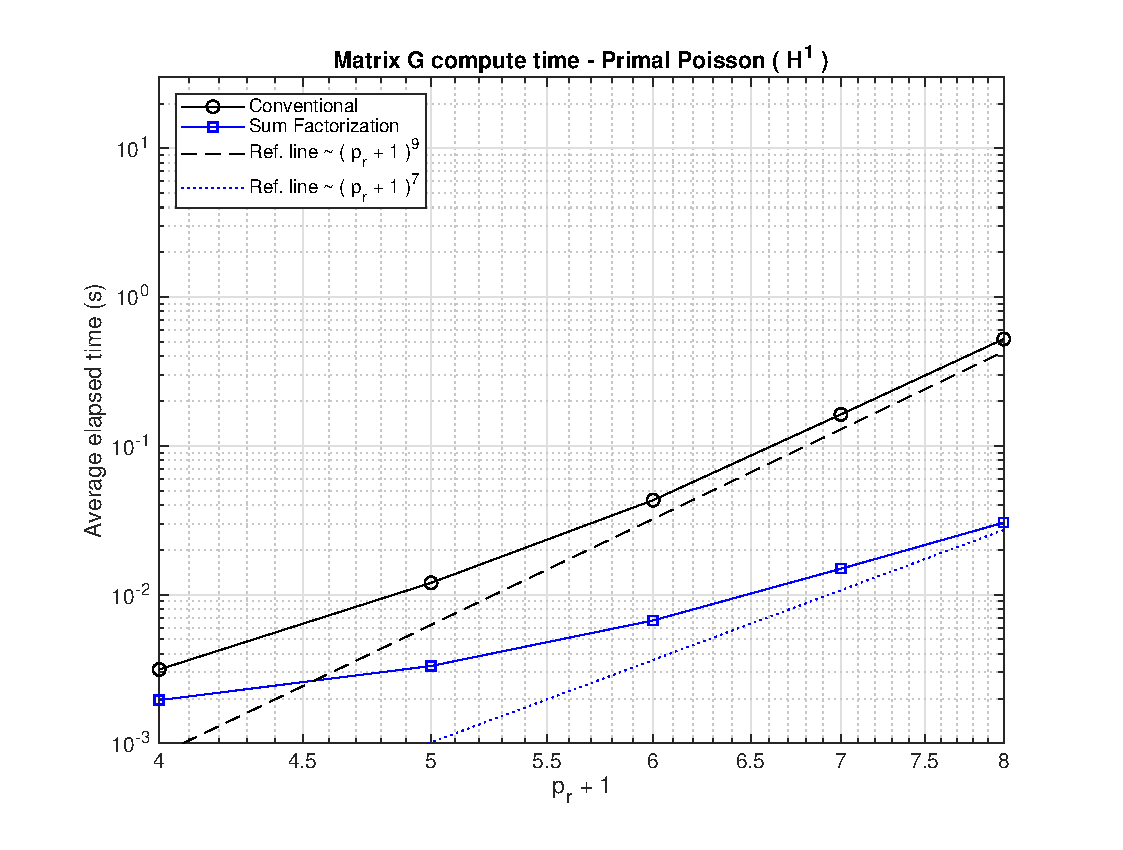
\includegraphics[width=11cm]{poisson_G.eps}
    \caption{Average computation time (seconds) of $\sfG^{\grad}$ in the Primal Poisson DPG implementation, for different polynomial orders and two integration algorithms with respect to $p_r+1$}
    \label{fig:results_poisson1}
\end{figure}

Additionally, Table \ref{tab:results_poisson2} and Figure \ref{fig:results_poisson2} show the average time for computing $\sfG$, $\sfB$ and $\sfell$ within the code's element subroutine (the component of the finite element code that constructs the element matrices), having fixed $\Delta p=2$. Since $\sfB$ and $\sfell$ are constructed using a conventional integration approach, this result intends to inform a closer estimate of the actual time savings when using sum factorization in a DPG computational solution. Notice that the reference line on this plot indicates that, in both cases, the trend is again approximately of ninth order.
% Here, it is more useful to see how expensive the process is for a given trial space order, then we plot with respect to $p_0$.
%
\begin{table}[ht]
    \centering
    \begin{tabular}{|c|c|c|c|c|}
    \hline
    $p_0$ & $\Delta p$ & $p_r$ & \textbf{Conventional} & \textbf{Sum factorization} \\
    \hline
1	&	2	&	3	&	3.55E-03	&	2.41E-03	\\
2	&	2	&	4	&	1.60E-02	&	7.20E-03	\\
3	&	2	&	5	&	6.62E-02	&	2.81E-02	\\
4	&	2	&	6	&	0.294	&	0.113	\\
5	&	2	&	7	&	1.01	&	0.404	\\
    \hline
    \end{tabular}
    \caption{Average computation time (seconds) of $\sfG^{\grad}$, $\mathsf{B}$, $\sfell$, in the Primal Poisson DPG implementation, for different polynomial orders and two integration algorithms}
    \label{tab:results_poisson2}
\end{table}
%
\begin{figure}[ht]
    \centering
    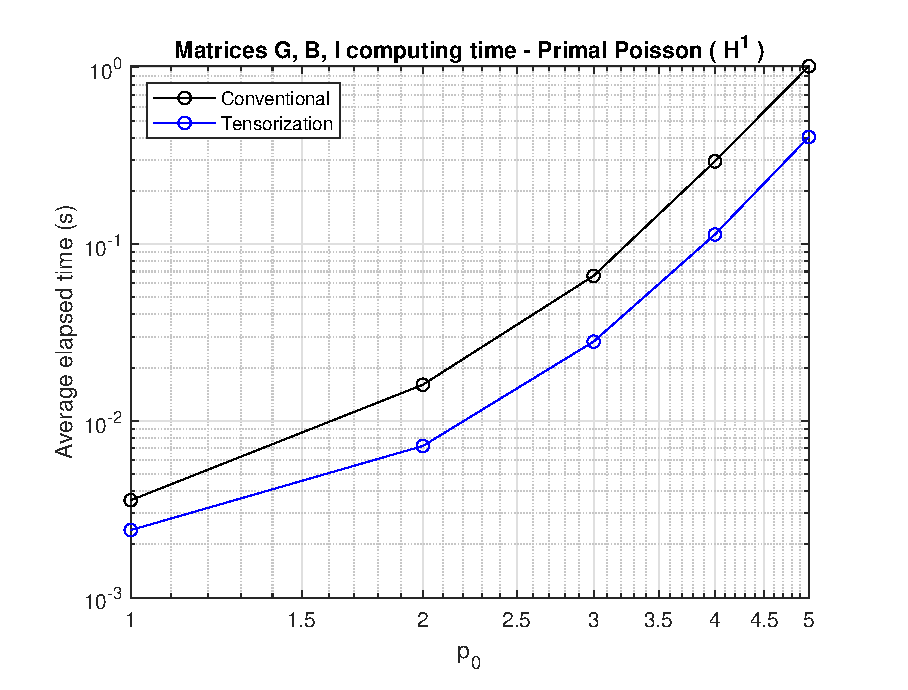
\includegraphics[width=11cm]{poisson_all.eps}
    \caption{Average computation time (seconds) of $\sfG^{\grad}$, $\mathsf{B}$, $\sfell$, in the Primal Poisson DPG implementation, for different polynomial orders and two integration algorithms with respect to $p_r+1$, with fixed $\Delta p=2$}
    \label{fig:results_poisson2}
\end{figure}
% 
 
\subsection{Primal formulation for Maxwell's equations}
% 
A second illustrative problem is the time-harmonic Maxwell's wave equation,
%
\begin{equation}
\curl{\color{red}{\left( \mu^{-1}\curl E \right)}} - \omega^2\epsilon E=\zI\omega J,
\label{maxwellpde}
\end{equation}
% 
where $E$ is the unknown electric field, $J$ is the imposed electric current, $\omega$ is the {\color{blue} angular frequency, and $\mu$ and $\epsilon$ are electromagnetic constants (the permeability and the permittivity, respectively)}. In terms of the abstract formulation (\ref{brokenvar}), the primal version of the broken variational form for (\ref{maxwellpde}) is

\begin{equation}
\begin{aligned}
    \scU&=\HSo(\curl,\Omega),\\
    \scW(\partial\mesh)&=\HSo^{-\onehalf}(\div,\partial\mesh)\\
    \scV&=\HSo(\curl,\mesh),\\
    b(E,F)&=(\mu^{-1}\curl E,\curl F)_\mesh-\omega^2(\epsilon E,F)_\mesh,\\
    \tilde{b}(\tilde{E},F)&=-\zI\omega\langle\tilde{E},F\rangle_{\partial\mesh},\\
    \ell(F)&=\zI\omega(J,F)_\mesh,
\end{aligned}
\label{maxwellbrokenprimal}
\end{equation}
%
where $E$ and $\tilde{E}$ are the trial variables, $F$ is the test variable, and $\langle\cdot,\cdot \rangle_{\partial\mesh}$ in this case represents the duality pairing between trace spaces $\HSo^{-\onehalf}(\div,\partial\mesh)$ and $\HSo^{-\onehalf}(\curl,\partial\mesh)$ \cite{BrokenForms15}.

The discrete enriched test subspace is $Q^{p_r}=T^{\curl}(\mcQ^{p_r-1,p_r,p_r}(\mcI^3) \times\mcQ^{p_r,p_r-1,p_r}(\mcI^3) \times\mcQ^{p_r,p_r,p_r-1}(\mcI^3))$. The Gram matrix that corresponds to this problem is the one for $H(\curl)$, hereby algorithms \ref{algo:hcurlconven} and \ref{algo:hcurltensor} are going to be compared.

Similarly to the previous case, we present results for the construction of the Gram matrix in Table \ref{tab:results_maxwell1} and Figure \ref{fig:results_maxwell1}. In this case, the time averages correspond to 20 runs. When taking into account also the integration of $\sfB$ and $\sfell$ the results are those shown in Table \ref{tab:results_maxwell2} and in Figure \ref{fig:results_maxwell2}.
%
\begin{table}[ht]
    \centering
    \begin{tabular}{|c|c|c|c|c|}
    \hline
    $p_0$ & $\Delta p$ & $p_r$ & \textbf{Conventional} & \textbf{Sum factorization} \\
    \hline
1	&	1	&	2	&	3.09E-02	&	3.41E-02	\\
1	&	2	&	3	&	4.22E-02	&	3.98E-02	\\
2	&	2	&	4	&	0.129	&	5.39E-02	\\
3	&	2	&	5	&	0.571	&	9.42E-02	\\
4	&	2	&	6	&	2.30	&	0.203	\\
5	&	2	&	7	&	7.82	&	0.464	\\
    \hline
    \end{tabular}
    \caption{Average computation time (seconds) of $\sfG^{\curl}$ in the Primal Maxwell DPG implementation, for different polynomial orders and two integration algorithms}
    \label{tab:results_maxwell1}
\end{table}
%
\begin{figure}[ht]
    \centering
    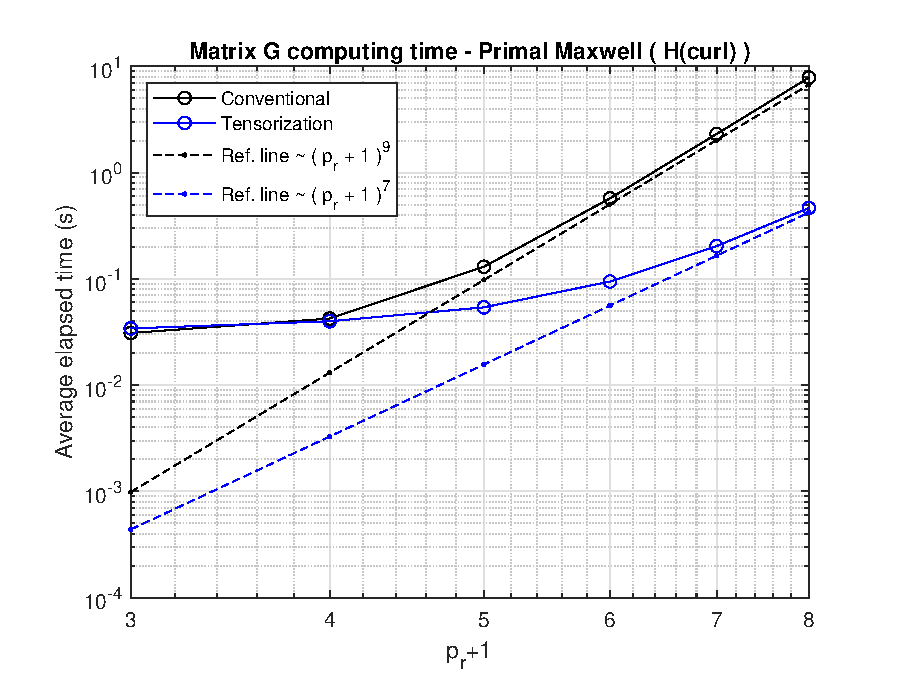
\includegraphics[width=11cm]{maxwell_G.eps}
    \caption{Average computation time (seconds) of $\sfG^{\curl}$ in the Primal Maxwell DPG implementation, for different polynomial orders and two integration algorithms with respect to $p_r+1$}
    \label{fig:results_maxwell1}
\end{figure}
%
\begin{table}[ht]
    \centering
    \begin{tabular}{|c|c|c|c|c|}
    \hline
    $p_0$ & $\Delta p$ & $p_r$ & \textbf{Conventional} & \textbf{Sum factorization} \\
    \hline
1	&	2	&	3	&	4.65E-02	&	3.37E-02	\\
2	&	2	&	4	&	0.167	&	7.75E-02	\\
3	&	2	&	5	&	0.889	&	0.340	\\
4	&	2	&	6	&	4.02	&	1.57	\\
5	&	2	&	7	&	15.36	&	6.02	\\
    \hline
    \end{tabular}
    \caption{Average computation time (seconds) of $\sfG^{\curl}$, $\sfB$, $\sfell$, in the Primal Maxwell DPG implementation, for different polynomial orders and two integration algorithms}
    \label{tab:results_maxwell2}
\end{table}
%
\begin{figure}[ht]
    \centering
    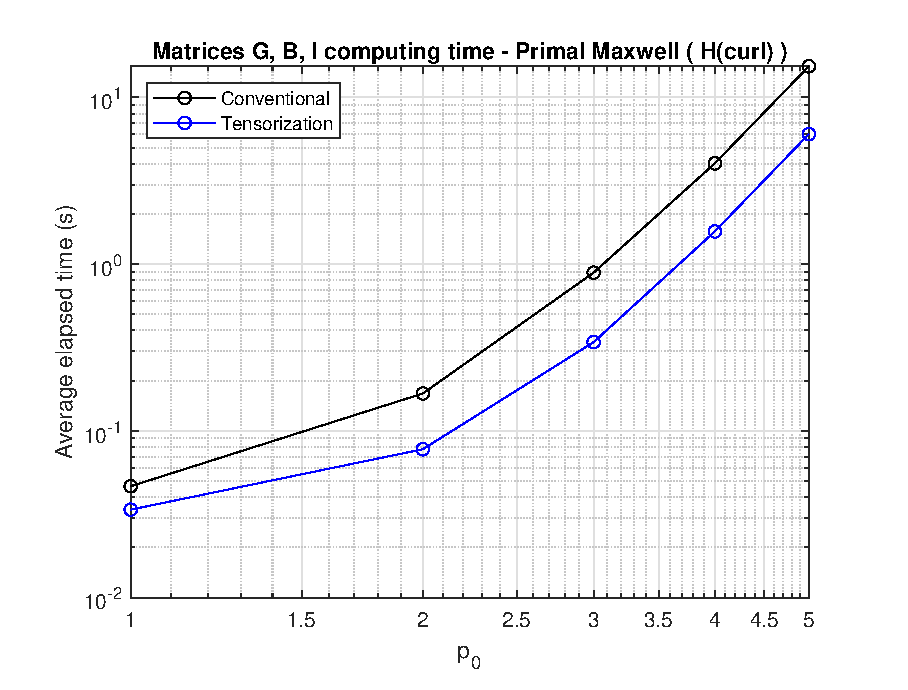
\includegraphics[width=11cm]{maxwell_all.eps}
    \caption{Average computation time (seconds) of $\sfG^{\curl}$, $\mathsf{B}$, $\sfell$, in the Primal Maxwell DPG implementation, for different polynomial orders and two integration algorithms with respect to $p_r+1$, with fixed $\Delta p=2$}
    \label{fig:results_maxwell2}
\end{figure}

\subsection{Acoustics and the ultraweak variational formulation}

The time-harmonic acoustics system of equations reads as follows:
%
\begin{equation}
    \left\{
    \begin{array}{ll}
        \zI\omega u + \nabla p &=0, \\
        \zI\omega p + \div u &=f,
    \end{array}
    \right.
\end{equation}
%
where $u$ is the velocity, $p$ the pressure, and $\omega$ the angular frequency. As a first order system, each equation can be tested independently (with broken test functions), and after applying integration by parts we get the so-called ultraweak variational formulation \cite{petrides2017adaptive}:
%
\begin{equation}
\begin{aligned}
    \scU&=\Leb^2(\Omega)\times\bLeb^3(\Omega),\\
    \scW(\partial\mesh)&=\HSo^{\onehalf}(\div,\partial\mesh)\times\HSo^{-\onehalf}(\div,\partial\mesh)\\
    \scV&=\HSo^1(\mesh)\times\HSo(\div,\mesh),\\
    b((p,u),(q,v))&=(\zI\omega u,v)_\mesh-(p,\div v)_\mesh+(\zI\omega p,q)_\mesh-(u,\nabla q)_\mesh,\\
    \tilde{b}((\tilde{p},\tilde{u}_n),(q,v))&=\langle\tilde{p},v\cdot n\rangle_{\partial\mesh}+\langle\tilde{u}_n,q\rangle_{\partial\mesh},\\
    \ell((q,v))&=(f,v)_\mesh,
\end{aligned}
\label{acousticsbrokenuw}
\end{equation}

Interestingly, this variational formulation is characterized by having its field trial variables lying in $L^2$ spaces. This immediately implies that there is no requirement on continuity across elements for the functions belonging to those spaces. Other variational formulations, where the trial space needs some kind of continuity (e.g. the primal formulations above), and therefore the handling of orientation and the distinction among the type of shape function (vertex, edge, face, interior) make the tensor-product decomposition less direct (see \cite{Fuentes2015}). Unlike those, the ultraweak variational formulation directly allows the correspondence of its discrete trial basis with tensor-product shape functions. As a result, we can apply very similar ideas as above to compute the volume integrals needed for $\sfB$ and $\sfell$, in addition to $\sfG$.

For a single element, notice that the stiffness matrix $\sfB$ arising from the bilinear functional in (\ref{acousticsbrokenuw}) can be computed as follows,
%
\begin{equation}
    \sfB_{IK}=(\zI\omega u_{K_{R}},v_{I_V})_\mcK-(p_{K_Q},\div v_{I_V})_\mcK+(\zI\omega p_{K_Q},q_{I_H})_\mcK -(u_{K_{R}},\nabla q_{I_H})_\mcK,
    \label{uw_stiffness}
\end{equation}
%
where $I$ is the product index of $I_H$ and $I_V$, $K$ is the product index of $K_Q$ and $K_{R}$, $p_{K_Q}\in Y^{p_0}$, $u_{K_R}\in (Y^{p_0})^3$, $q_{I_H}\in W^{p_r}$, and $v_{I_V}\in V^{p_r}$. By mapping to the master hexahedron and using the Piola transformations we obtain:
%
\begin{equation}
    \sfB_{IK}=\int\limits_{\hatK} \left(
                \zI\omega \hat{u}_{K_{R}}^\T\mcJ\hat{v}_{I_V}|\mcJ|^{-1}-\hat{p}_{K_Q},\hat{\div} \hat{v}_{I_V}|\mcJ|^{-1}
                +\zI\omega \hat{p}_{K_Q}\hat{q}_{I_H}-\hat{u}_{K_{R}}^\T\mcJ^{-\T}\hat{\nabla} \hat{q}_{I_H}
                \right)d^3\bsxi.
    \label{uw_stiffness_master}
\end{equation}

For each term of (\ref{uw_stiffness_master}), we can express the involved shape functions as tensor products of univariate polynomials, and develop similar algorithms as the ones derived above. A similar idea can be applied for the simpler situation of $\sfell$.

Additionally, the choice of a special norm in the ultraweak formulation is of great benefit to be able to control the solution error in the desired trial norm \cite{DPGOverview}. Such a norm is the so-called \textit{adjoint graph norm}, with a corresponding inner product that is defined as follows,
%
\begin{equation}
\begin{aligned}
    \left((\delta q,\delta v),(q,v)\right)_{\scV}=&
    [\omega^2+\alpha](\delta q,q)_\mesh+(\nabla \delta q,\nabla q)_\mesh
    -\zI\omega(\div \delta v,q)_\mesh +\zI\omega(\delta v, \nabla q)_\mesh \\
&    +\zI\omega(\delta q,\div v)_\mesh -\zI\omega(\nabla\delta  q,v)_\mesh+ 
    [\omega^2+\alpha](\delta v, v)_\mesh+(\div \delta v,\div v)_\mesh,\ \ \forall (\delta q,\delta v),(q,v)\in\scV.
\end{aligned}
\label{acoustics_adjoint_norm}
\end{equation}

In (\ref{acoustics_adjoint_norm}), $\alpha$ is some positive real number that is used as a correction due to the fact of using broken test spaces \cite{petrides2017adaptive}. Notice that four terms in this inner product were already studied in the $H^1$ and $H(\div)$ spaces. The remaining four terms form a Hermitian array, so that we need to implement only two of them. Considering a single element, the third and fourth terms of (\ref{acoustics_adjoint_norm}) lead to
%
\begin{equation}
    -\zI\omega(\div \delta v,q)_\mcK +\zI\omega(\delta v, \nabla q)_\mcK=
    \zI\omega\int\limits_{\hatK}\left[-(\hat{\div}\hat{\delta v})(\hat{q})+ (\hat{\delta v})^\T(\hat{\nabla}\hat{q}) \right]d^3\bsxi,
\label{adjoint_norm_terms}
\end{equation}
%
after implementing the respective Piola maps. Finally, besides using Algorithms \ref{algo:h1tensor} and \ref{algo:hdivtensor} for the four associated terms in (\ref{acoustics_adjoint_norm}), an analogous sum factorization algorithm must be built for the two integrals in (\ref{adjoint_norm_terms}).

This problem was solved using both conventional integration and tensor-product based integration, translating the ideas above for the stiffness matrix, the load vector and the Gram matrix produced by the adjoint graph norm, into the code. Table \ref{tab:results_acoustics} and Figure \ref{fig:results_acoustics} show the results of the average computing time (of 20 runs) of $\sfG$, $\sfB$, and $\sfell$, for several polynomial degrees. Here, because of the different trends observed, two reference lines are presented, one of ninth order and one of seventh order.
%
\begin{table}[ht]
    \centering
    \begin{tabular}{|c|c|c|c|c|}
    \hline
    $p_0$ & $\Delta p$ & $p_r$ & \textbf{Conventional} & \textbf{Sum factorization} \\
    \hline
    1	&	1	&	2	&	1.48E-03	&	7.15E-04	\\
    1	&	2	&	3	&	1.05E-02	&	3.40E-03	\\
    2	&	2	&	4	&	7.46E-02	&	9.62E-03	\\
    3	&	2	&	5	&	0.437	&	2.84E-02	\\
    4	&	2	&	6	&	1.900	&	8.08E-02	\\
    5	&	2	&	7	&	6.985	&	0.214	\\
    6	&	2	&	8	&	21.88	&	0.496	\\
    \hline
    \end{tabular}
    \caption{Average computation time (seconds) of $\sfG$, $\sfB$ and $\sfell$ in the ultraweak acoustics DPG implementation, for different polynomial orders and two integration algorithms}
    \label{tab:results_acoustics}
\end{table}
%
\begin{figure}[ht]
    \centering
    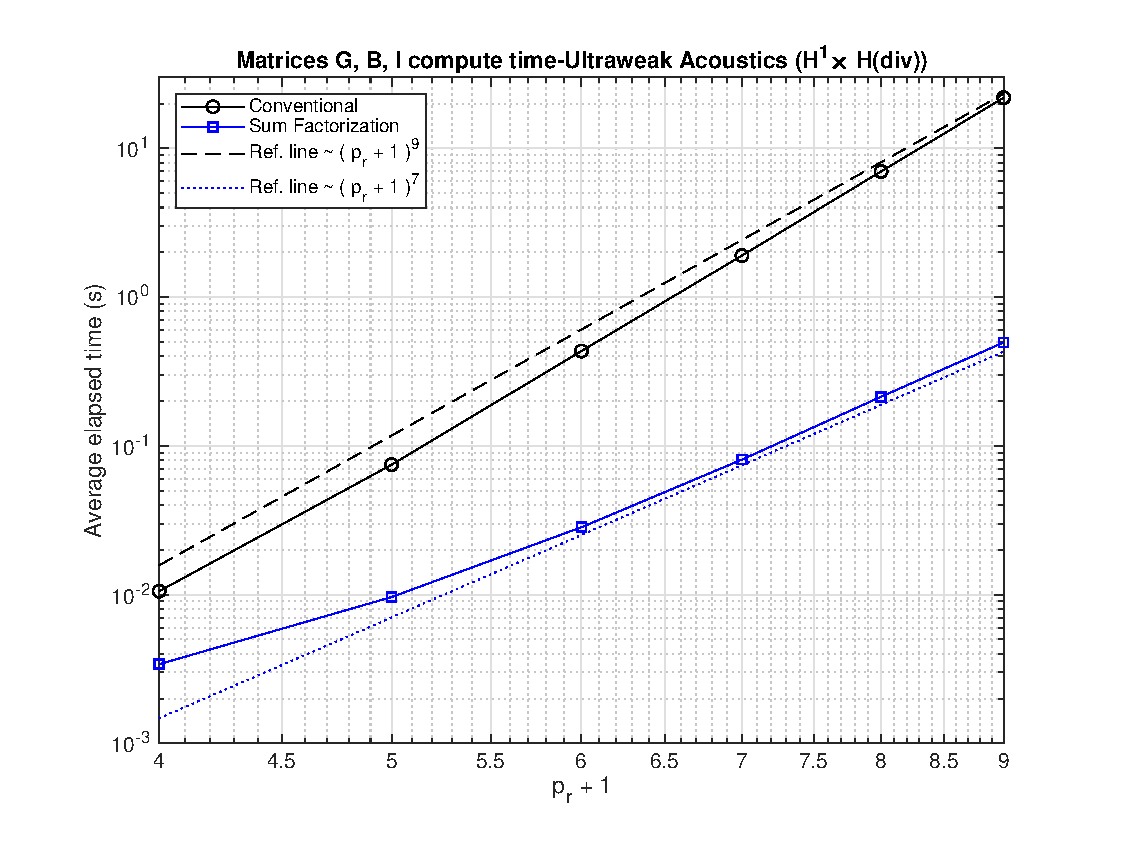
\includegraphics[width=11cm]{acoustics.eps}
    \caption{Average computation time (seconds) of $\sfG$, $\mathsf{B}$, $\sfell$, in the ultraweak acoustics DPG implementation, for different polynomial orders and two integration algorithms with respect to $p_r+1$, with fixed $\Delta p=2$}
    \label{fig:results_acoustics}
\end{figure}

\subsection{Discussion}

The results observed above allow to identify several achievements, while also make clear what aspects need improvement. Notice that all five plots have the same scales in their axes in order to facilitate visual comparison.

Firstly, Figures \ref{fig:results_poisson1} and \ref{fig:results_maxwell1} communicate well that the expected asymptotic reference lines approach the numerical experiments results as $p_r$ increases. Unlike the dashed reference line (corresponding to $(p_r+1)^9$), which is almost parallel to the plot for conventional integration, the fine dotted line (corresponding to $(p_r+1)^7$) seems to grow slightly faster than the data for the sum factorization results. It may be expected that at higher polynomial degrees the rate becomes closer to 7, but at the moment the important outcome is that the integration of $\sfG$ indeed became two orders of magnitude faster.

% This is more noticeable in the case of Poisson, in which, because of dealing with a $H^1$-only Gram matrix and a smaller set of auxiliary functions is required (in algorithm \ref{algo:h1tensor}), then the final accumulation statement quickly begins to dominate the computational complexity as the polynomial order rises. On the other hand, the case of Maxwell's equation required the use of algorithm \ref{algo:hcurltensor}, which has intermediate accumulation statements that are comparable in cost to the final one when $p_r$ is not very high. However, on Figure \ref{fig:results_maxwell1} the last three values of polynomial order indicate that the computing time clearly develops at a slower rate than in the conventional case, which indeed looks quite close to the trend line $~(p_r+1)^9$.

As a second observation, we see that Figures \ref{fig:results_poisson2} and \ref{fig:results_maxwell2} reveal that, when looking at the elapsed time of computing all the matrices, the sum factorization approach overcomes the performance of the conventional algorithm at all degrees $p_r$. Such a result is also visible in Tables \ref{tab:results_poisson2} and \ref{tab:results_maxwell2}, in which the difference between columns 4 and 5 correspond to the actual time saving when going from the conventional integration scheme to the herein introduced algorithm, for every time the element subroutine is invoked in a DPG code. For the highest values of $p_r$, this saving can be of the order of a second per element in Poisson, or 9 seconds in Maxwell, therefore leading to a big reduction of computation time when a refined mesh is in use. It can be seen nevertheless that the complexity rate for the compute time of all the matrices, in both types of integration, is still 9. This happens because computing the stiffness matrix $\sfB$ with the conventional algorithm has a leading term of $\mcO((p_0+1)^9)$ in its computational complexity, which will obviously begin dominating the cost of all the integration as $p_0$ grows.

Earning all the advantages of sum factorization for numerical integration has therefore the requirement of finding a good procedure for the construction of $\sfB$ and $\sfell$. Such a procedure must be able to take profit of the nesting of integrals, as developed above for so diverse situations, for multiple variational formulations. 

For the ultraweak formulation, that was clearly observed. In that case, there was a way to extend the ideas of sum factorization and take advantage of them, as noticed in Figure \ref{fig:results_acoustics}. There, it can be seen that the complexity rates were successfully taken to the desired order.
% However, for the first two problems, the effect of not having available a more efficient algorithm for these matrices can be appreciated in the last points of Figures \ref{fig:results_poisson2} and \ref{fig:results_maxwell2}, where, despite relatively big savings in the overall computing time of the matrices under study, it is clear that the rate of the tensor-product-based algorithm is similar to that of the conventional algorithm. This happens because computing the stiffness matrix $\sfB$ in this way has a computational complexity leading term of $\mcO((p_0+1)^9)$, which will obviously begin dominating the cost of all the integration as $p_0$ grows.

As a closing remark, we can state that having proposed and utilized a tensor-product-based algorithm for the integration of less usual Gram matrices, like that of $H(\curl)$ or the adjoint-graph inner product for $H^1\times H(\div)$, proved to be very useful regarding the really meaningful relative savings: 16 times faster when $p_0=5$ and $\Delta p=2$, in Maxwell's primal form; or 44 times faster in the ultraweak formulation for acoustics with $p_0=6$ and $\Delta p=2$. This kind of benefit is thereby expected to extend to the rest of energy spaces and inner products frequently used in DPG and other FE methods.